\chapter{Literature Review}
\paragraph{}
This section discusses some papers that are relevant to the project's study regarding the application of model predictive controllers for self-driving vehicle control.

\section{P. Falcone et al (2007) [1]}
\paragraph{}
This paper discusses a MPC approach for controlling an active front steering system in an autonomous vehicle. A large emphasis is placed on precise modeling of the vehicle dynamics, including detailed models of the wheel equations of motion and tire forces as a function of longitudinal slip and tire slip angles. The model defines a hierarchical framework for the control task involving four modules:
\vspace{-2.5mm}

\begin{enumerate}[label=(\arabic*), itemsep=-0.3em]
    \item trajectory/mode generator: performs offline pre-computation of the vehicle trajectory along with conditions for operation mode change (e.g., switching between different fuel sources in a hybrid electric vehicle)
    \item trajectory/mode replanning: re-computes the trajectory online based on current measurements while executing the driving task, at fixed points or on the occurrence of certain events (e.g., tracking errors exceeding pre-defined bounds, adverse weather, etc)
    \item low-level control system: commands the vehicle actuators based on sensor measurements, states and parameter estimations, with an objective of keeping the vehicle as close to the planned trajectory
    \item vehicle and environment model: process plant that takes into account external disturbances and converts the control outputs $u, X$ into vehicle state outputs $Y$
\end{enumerate}

\paragraph{}
The paper discusses three types of MPC controllers for active steering controller design, all of which are capable of incorporating the highly non-linear Pacejka tire model that has been used for vehicle dynamics modeling. All the control systems are subjected to the same driving task of a vehicle performing a double lane change maneuver on a slippery road. Controller A is a non-linear MPC controller with a sample time $T = 0.05\text{ s}$, prediction horizon $H_p=7$ control intervals and control horizon $H_c=3$ control intervals. The values of the yaw angle and yaw rate are limited to $\pm 10\degree$ and $\pm 1.5\degree$ respectively. Figure 3.1 illustrates the response of controller A, with the three plots indicating the vehicle's lateral position, yaw angle and yaw rate respectively.

\begin{figure}[H]\label{fig3.1}
\centering 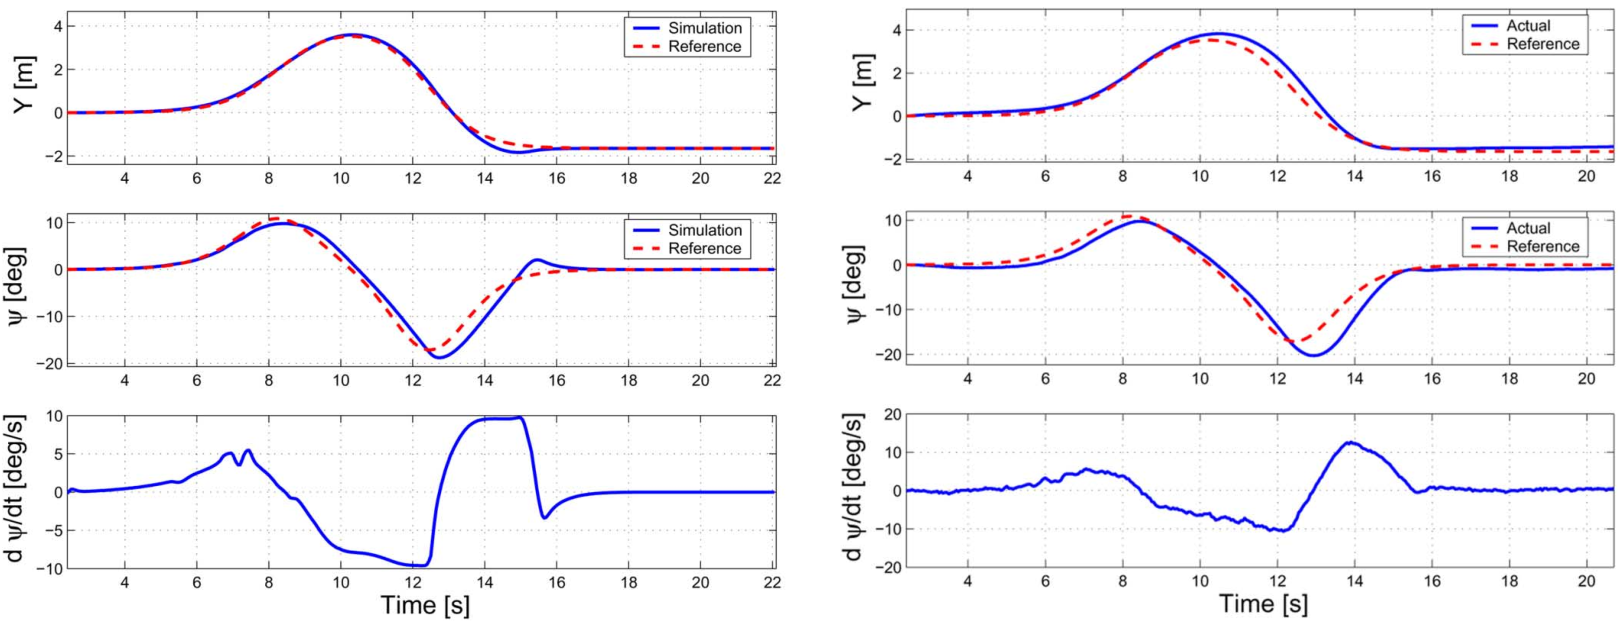
\includegraphics[width=\textwidth]{Images/paper1_controllerA_response.png}
\caption{Comparison of Simulation and Experimental Response for Controller A (Entry Speed = 7 m/s)}
\end{figure}

\paragraph{}
Controller B is a linear time-variant MPC controller with a sample time $T = 0.05\text{ s}$, prediction horizon $H_p=25$ control intervals and control horizon $H_c=10$ control intervals. The values of the yaw angle and yaw rate are limited to $\pm 10\degree$ and $\pm 0.85\degree$ respectively. Further, the rate of angular acceleration (about the instantaneous center of rotation, as defined in section 2.1.1) is also limited to $\pm 2.2\degree$. Controller C has the same architecture as controller B with $H_c = 1$ control interval. Figure 3.2 illustrates the responses of controller B.

\begin{figure}[H]\label{fig3.2}
\centering 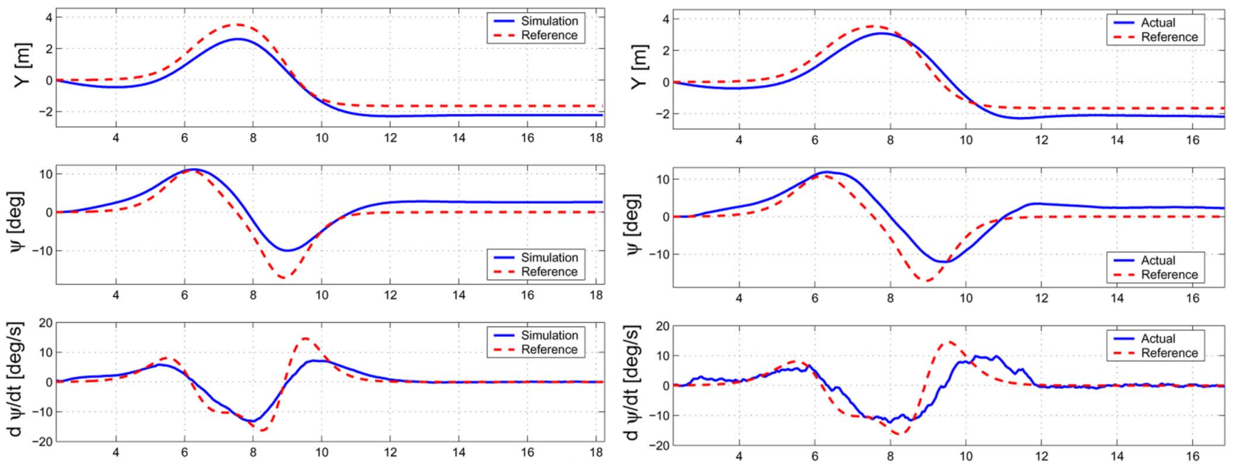
\includegraphics[width=\textwidth]{Images/paper1_controllerB_response.png}
\caption{Comparison of Simulation and Experimental Response for Controller B (Entry Speed = 10 m/s)}
\end{figure}

\paragraph{}
The plots of the responses of controller C have not been provided, however, the paper compares the maximum tracking errors. It is inferred from this analysis that the performance of controller C is slightly worse as compared to controller B. However, it is able to stabilize the vehicle at high speeds.

\paragraph{}
Both the non-linear and linear time-variant MPC approaches suffer from the difficulty in verifying the optimization code and computing the worst case computational time. The results of this paper open the route to research activities to enlarge the range of conditions for which non-linear MPC becomes real-time implementable.

\section{T. Takahama et al (2010) [2]}
\paragraph{}
This paper, in collaboration with \textit{Hitachi Automotive Systems Ltd} and \textbf{The Mathworks GK}, presents a design method for a model predictive controller with a low computational cost for a practical ACC system. The ACC task consists of maintaining a desired inter-vehicle distance while following the desired velocity as much as possible. 

\paragraph{}
The paper discretizes the non-linear vehicle dynamics model to construct a simple MPC predictor with a low dimension. The linear optimization problem results in a quadratic objective function, similar to the one discussed in Section 2.3.2. The inter-vehicle distance is emphasized as the main objective by setting the weights of the control inputs and rate of change of the control inputs to zero. 

\paragraph{}
The controller's sampling time is $T_s=0.05\text{ s}$, and the prediction and control horizons are $p = 20$ and $c = 1$ control intervals respectively. The control horizon is chosen to be small on purpose to reduce the computational load on the processor. The control input and its rate of change are bounded by the values $\pm 2.5$ and $\pm 1.5$ respectively. Figure 3.3 shows a comparison of the MPC simulation response (left) to the response of a linear quadratic regulator system (right).

\begin{figure}[H]\label{fig3.3}
\centering 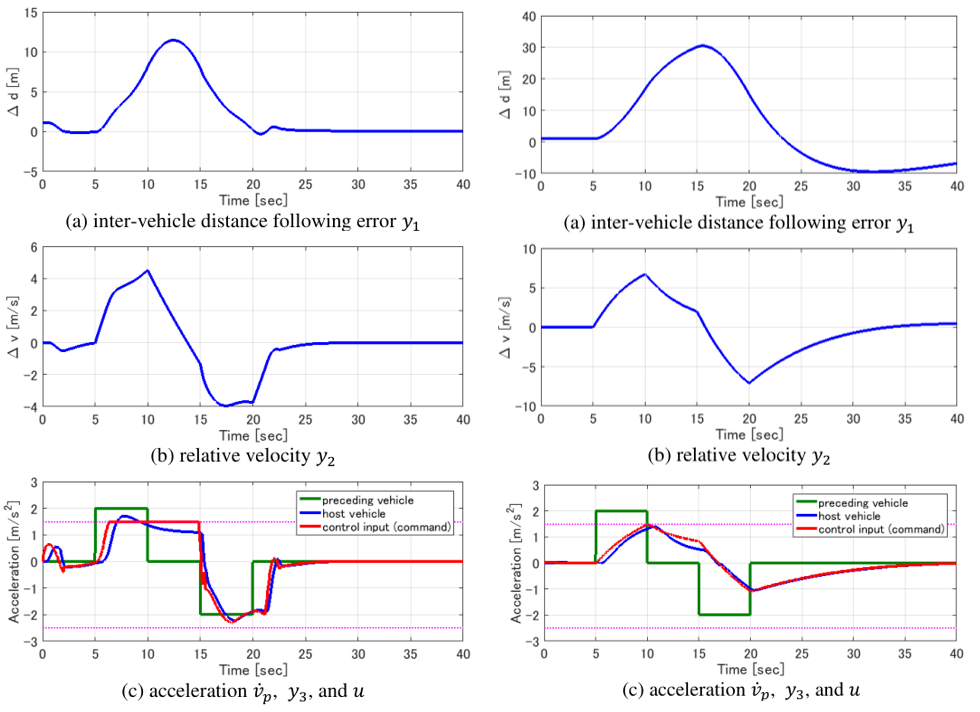
\includegraphics[width=\textwidth]{Images/paper2_model_performance.png}
\caption{Comparison of MPC and LQR Simulation Responses}
\end{figure}

\paragraph{}
The results clearly show that the MPC control system has a better output response - the plant outputs $y_i$ and $y_2$ converges to zero, and the ego vehicle states and control inputs offer a better tracking response. The LQR system displays a tardy response due to the small feedback gain, which is used to reduce the overall magnitude of the control inputs for linear controllers. The better performance of the MPC controller is expected since it can deal with explicit actuator constraints directly within the framework of the optimization problem. 

\section{T. M. Vu et al (2010) [3]}
\paragraph{}
This paper presents the design of a non-linear model predictive controller subject to hard constraints. The same model is later subjected to softened constraints, which is likely to provide a higher probability of finding the optimal control action and maintaining system stability. The paper makes use of a slightly different vehicle dynamics model compared to the bicycle model discussed in Section 2.1.1. It makes use of the distance between the front and rear wheel centres, called the wheelbase, $l$, and the rolling radius of the wheels $r$. This leads to the dynamics equation as follows:
$$\begin{bmatrix}[1]
    \dot{x}\\ \dot{y}\\ \dot{\theta}\\  \dot{\phi}\\
\end{bmatrix}=\begin{bmatrix}[1]
    \cos\theta\cos\phi\\ \sin\theta\cos\phi\\ \frac{\tan\phi}{l}\\  0\\
\end{bmatrix}rv_1 + \begin{bmatrix}[1]
    0\\ 0\\ 0\\  1\\
\end{bmatrix}v_2$$

\begin{figure}[H]\label{fig3.4}
\centering 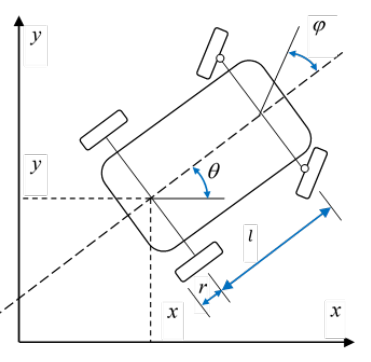
\includegraphics[scale=0.8]{Images/paper3_vehicle_dynamics_model.png}
\caption{A Different Vehicle Model used for Dynamics Modeling}
\end{figure}

\paragraph{}
The paper then discusses the implementation of the two non-linear MPC models involving hard and soft constraints. In the model involving softened constraints, some constraints on certain physical parameters are relaxed. However, the objective function for this model contains an additional term which penalizes the violations of the softened constraints (much like a reinforcement learning agent) - if the penalty term is reasonably high, the model returns the free constrained solution if one exists. Figures 3.5 and 3.6 illustrate the tracking response of the two models along a circular path and an interpolated polynomial path respectively.

\begin{figure}[H]\label{fig3.5}
\centering 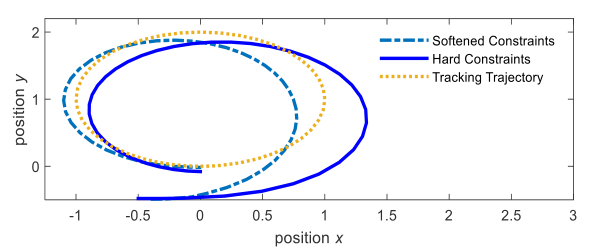
\includegraphics[scale=1]{Images/paper3_circular_path_tracking.png}
\caption{Trajectory Tracking Responses of the Models for a Circular Path}
\end{figure}

\begin{figure}[H]\label{fig3.6}
\centering 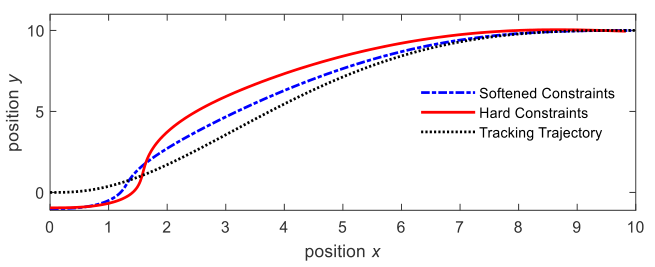
\includegraphics[scale=0.92]{Images/paper3_trajectory_tracking.png}
\caption{Trajectory Tracking Responses of the Models for an Interpolated Polynomial Path}
\end{figure}

\paragraph{}
The results show that the tracking performance of the non-linear MPC model with softened constraints is better compared to the one with hard constraints. This is expected since the model with soft constraints is likely to slightly violate some constraints in favour of a response with smaller tracking errors.

\paragraph{}
Finally, the paper briefly discusses the effect of prediction horizon on the two models. In case of a short prediction horizon, the model with hard constraints results in tighter control actions and a response that deviates significantly from the reference trajectory as well as the response of the model with softened constraints. As the prediction horizon is lengthened, both the systems become looser and more flexible, leading to a much closer tracking response between the two models. 